\chapter{編輯原子結構}\label{ch:modeling}

\chapterlead{一個可用於計算的結構，既要有正確的原子種類和位置，也要恰當地表達週期性、連線關係與晶胞。本章從檢視矽晶胞開始，介紹選擇、編輯和儲存模型的方法，再透過超胞、空位、芳香分子和乙醇的例子，把常用工具串成完整的操作過程。}

\section{認識結構模型}

\subsection{晶體與分子的區別}
\index{Fenzi jianmo@分子建模}

晶體模型用一個晶胞和其中的原子描述週期排列的物質。晶胞的三條邊由晶格向量 $\mathbf a$、$\mathbf b$、$\mathbf c$ 表示，它們決定晶胞的大小和形狀。晶格向量不必互相垂直；在斜晶胞中，沿晶格方向移動與沿螢幕上的水平、豎直方向移動是兩回事。

分子模型通常是一組有限的原子，並具有明確的化學鍵連線關係。繪製一個乙醇分子時，需要同時說明哪些原子相連、連線的是單鍵還是雙鍵。螢幕上看起來相近的兩個原子，並不一定已經建立了用於分子編輯的連線關係。因此，在分子建模中，應把原子位置與化學鍵作為同一個模型的兩個方面一起檢查。

啟用三維結構文件後，工具區會根據當前物件顯示\ui{晶體建模}或\ui{分子建模}。晶體建模提供晶胞、對稱性、缺陷和表面等工具；分子建模提供草繪、化學性質、片段與幾何調整。命令是否可用還取決於當前選擇。例如，設定距離需要兩個原子，設定角度需要三個原子，只有一個原子的選擇不能用於這兩個命令。

開始編輯時，先從側欄開啟\ui{專案瀏覽器}，展開 \ui{Structure} 並雙擊目標結構，再選擇頂部相應的建模頁面。如果專案樹未顯示，可在側欄面板庫的\ui{開啟面板}視窗選擇\ui{專案瀏覽器}。側欄負責顯示和收起工作面板，頂部建模頁面提供本章使用的結構命令。

\subsection{笛卡爾座標與分數座標}

笛卡爾座標直接表示原子在空間中的位置，建模介面通常以埃（\AA）為單位。分數座標則表示沿三條晶格向量的比例。若分數座標為 $(u,v,w)$，原子的位置就是 $u\mathbf a+v\mathbf b+w\mathbf c$。這三個數沒有長度單位；它們回答的是“沿每條晶格向量走多少”，而不是“沿全域性座標軸走多少埃”。

為讀懂晶格輸入表格，可以把三條向量按行排成一個矩陣：
\[
 A=\begin{bmatrix}
 a_x&a_y&a_z\\
 b_x&b_y&b_z\\
 c_x&c_y&c_z
 \end{bmatrix},\qquad
 \mathbf f=(u,v,w),\qquad \mathbf r=(x,y,z).
\]
矩陣的第一行是 $\mathbf a$，第二、三行依次是 $\mathbf b$、$\mathbf c$；每行中的三列才是全域性 $x,y,z$ 分量。本書將座標寫成行向量，因此兩種座標的轉換為
\begin{equation}
 \mathbf r=\mathbf f A,\qquad \mathbf f=\mathbf r A^{-1}.
 \label{eq:row-lattice-coordinates}
\end{equation}
這裡 $A^{-1}$ 是整個晶格矩陣的逆矩陣，不能把表格中的每個數分別取倒數。晶格三行所定義的晶胞應有非零體積，才能由笛卡爾位置求回唯一的分數座標。

以一組便於手算的晶格說明：令 $\mathbf a=(4,0,0)$、$\mathbf b=(1,3,0)$、$\mathbf c=(0,0,6)$，單位均為\AA。分數座標 $(0.5,0.5,0)$ 對應
\[
 \mathbf r=0.5(4,0,0)+0.5(1,3,0)
          =(2.5,1.5,0)\,\text{\AA}.
\]
沿 $\mathbf b$ 走一半，同時包含全域性 $x$ 方向的 $0.5\,\text{\AA}$ 和 $y$ 方向的 $1.5\,\text{\AA}$。所以斜晶胞中的第二個分數分量，不能直接當作全域性 $y$ 座標。圖\ref{fig:round10-fractional-cartesian}將這一次相加畫成兩段相接的箭頭。

\begin{figure}[!htb]
\centering
\begin{tikzpicture}[x=1mm,y=1mm,font=\sffamily\small]
 \fill[paleblue] (8,6)--(56,6)--(68,42)--(20,42)--cycle;
 \draw[teal,line width=.7pt] (8,6)--(56,6)--(68,42)--(20,42)--cycle;
 \draw[->,>=stealth,muted] (8,6)--(84,6) node[right] {$x$};
 \draw[->,>=stealth,muted] (8,6)--(8,49) node[above] {$y$};
 \draw[->,>=stealth,brand,line width=1pt] (8,6)--(32,6);
 \draw[->,>=stealth,brand,line width=1pt] (32,6)--(38,24);
 \draw[->,>=stealth,teal,line width=.8pt] (8,6)--(38,24);
 \draw[dashed,muted] (38,24)--(38,6);
 \fill[brand] (38,24) circle (1.2);
 \node[anchor=north,text=brand] at (22,5) {$u\mathbf a$};
 \node[anchor=west,text=brand] at (38,14) {$v\mathbf b$};
 \node[anchor=south east,text=teal] at (25,16) {$\mathbf r$};
 \node[anchor=north east] at (7,5) {$O$};
 \node[anchor=west,text=brand] at (42,27) {$\mathbf f=(u,v,0)$};
 \node[anchor=west,text=muted,font=\sffamily\footnotesize] at (78,35) {晶胞在平面内的截面};
 \node[anchor=west,text=muted,font=\sffamily\footnotesize] at (78,28) {箭头相加得到位置};
 \node[anchor=north,text=teal] at (54,4) {$\mathbf a$};
 \node[anchor=east,text=teal] at (15,31) {$\mathbf b$};
\end{tikzpicture}
\caption{分数坐标与笛卡尔位置的关系（二维示意）。$u\mathbf a$ 与 $v\mathbf b$ 相加得到 $\mathbf r$；斜晶胞的 $\mathbf b$ 方向同时含有全局 $x$ 和 $y$ 分量。}
\label{fig:round10-fractional-cartesian}
\end{figure}


在邊長為 $5\,\text{\AA}$ 的立方晶胞中，$(0.5,0,0)$ 則對應沿 $\mathbf a$ 前進 $2.5\,\text{\AA}$。兩種例子的區別來自晶格，而不是座標轉換規則不同。編輯時若保持 $\mathbf f$ 不變而改變 $A$，原子通常會隨晶胞移動；若希望原子在空間中的位置不動，則需保留 $\mathbf r$，並用新晶格重新求 $\mathbf f$。第\ref{ch:modeling-tools}章的\ref{sec:lattice-transform-reference}節介紹這兩個選項。

\begin{table}[!htb]
\centering\small
\begin{tabularx}{\linewidth}{llX}
\toprule
符號 & 單位 & 在引數中的含義\\
\midrule
$A$ & \AA & 晶格矩陣，三行依次為 $\mathbf a,\mathbf b,\mathbf c$。\\
$\mathbf f$ & 無量綱 & 沿三條晶格向量的比例，即分數座標。\\
$\mathbf r,\mathbf p$ & \AA & 笛卡爾位置，以及旋轉錨點或鏡面上的點。\\
$\mathbf n,\hat{\mathbf n}$ & 方向 & 非零方向向量及其單位向量；只看方向時不以\AA 填長度。\\
$\theta$ & 度 & 對話方塊中的轉角，正角按右手定則。\\
$S$ & 整數 & 定義新晶格的超胞變換矩陣。\\
$N,V$ & 個、\AA$^3$ & 模型獨立位點數與晶胞體積。\\
$\varepsilon_a,\varepsilon_b,\varepsilon_c$ & 無量綱 & 沿三條晶格向量的相對伸縮量。\\
\bottomrule
\end{tabularx}
\caption{閱讀建模公式時常用的符號。座標和錨點使用長度，方向向量只指定朝向；兩者在對話方塊中有不同作用。}
\label{tab:round10-modeling-symbols}
\end{table}


選擇一個原子後，三維檢視內的原子資訊區域可幫助核對位置。晶體中的週期映像可能位於相鄰晶胞，其中的映像偏移用於指出這一點。進行數值編輯時，應先確認座標型別，再輸入三個分量。不能把 $0.5\,\text{\AA}$ 與半個晶格向量混用。

\Needspace{7\baselineskip}
\begin{notebox}{原子序號}
建模對話方塊中的原子序號從 1 開始。序號用於指定當前文件中的位點，與元素的原子序數不同。例如，原子序號 6 可以指第六個矽原子，並不表示碳。改變模型的原子數或重新排序後，應重新核對需要編輯的位點。
\end{notebox}

\section{示例：檢視一個矽晶胞}

本例使用手冊示例中的 \mbox{\file{Si.poscar}}。該檔案包含 8 個矽原子，立方晶胞邊長約為 $5.46873\,\text{\AA}$。該晶格常數用作建模練習的初始引數。

第\ref{ch:workflows}章的實際矽計算使用另一份 \file{silicon.cif}，邊長約為 $5.44370\,\text{\AA}$。兩份檔案都包含 8 個矽位點，但晶格常數不同；本章檢查超胞倍數時使用 \mbox{\file{Si.poscar}}，比較計算能量時則按計算章節指定檔案開始。

本節沿用第\ref{ch:workspace}章儲存的 \file{Si-introduction.ks}，再匯入建模用的 \file{Si.poscar}。專案樹中會同時保留原來的 \file{silicon} 與新匯入的 \file{Si}；以下操作均在 \file{Si} 文件中完成。完成建模後另存專案，便能保留第一個練習的原檔案。

\begin{steps}
  \item 開啟 \file{Si-introduction.ks}，將 \file{Si.poscar} 匯入專案，開啟新結構 \file{Si} 的三維文件，等待原子、晶胞和資訊區域顯示完成。
  \item 用滑鼠左鍵拖動旋轉檢視，用滾輪縮放。先觀察整個晶胞，再放大到能夠區分單個原子的位置。
  \item 單擊一個原子，檢視位點序號、元素和座標。再次選擇另一原子，觀察資訊如何隨選擇改變。
  \item 使用檢視工具欄的晶軸按鈕，從不同晶格方向觀察結構。在非正交晶胞中，晶格軸與其對應的倒易軸方向可能不同；這個區別將在觀察傾斜表面時更明顯。
  \item 按空格鍵重新居中並適配縮放。旋轉檢視只改變觀察方向，不改變模型中的原子位置。
\end{steps}

圖\ref{fig:si-periodic-image-inspection}顯示 Site 7 週期映像的原子資訊卡。卡片中的分數座標與\ui{Image}偏移相減，可得到模型內的分數座標：
\[
 (0.750,0.250,1.250)-(0,0,1)=(0.750,0.250,0.250).
\]
映像偏移表示沿 $\mathbf c$ 平移一個晶胞。卡片中的笛卡爾座標給出這一顯示映像的位置。座標超出 0 到 1，並不表示模型多出一個獨立位點。圖中的檢視器摘要為 8 sites、41 atoms，後一個數字包含顯示映像。

\begin{figure}[!htb]
\centering
% 原图3024×1758；完整卡(55,743,845,1305)，790×562；79mm约254ppi。
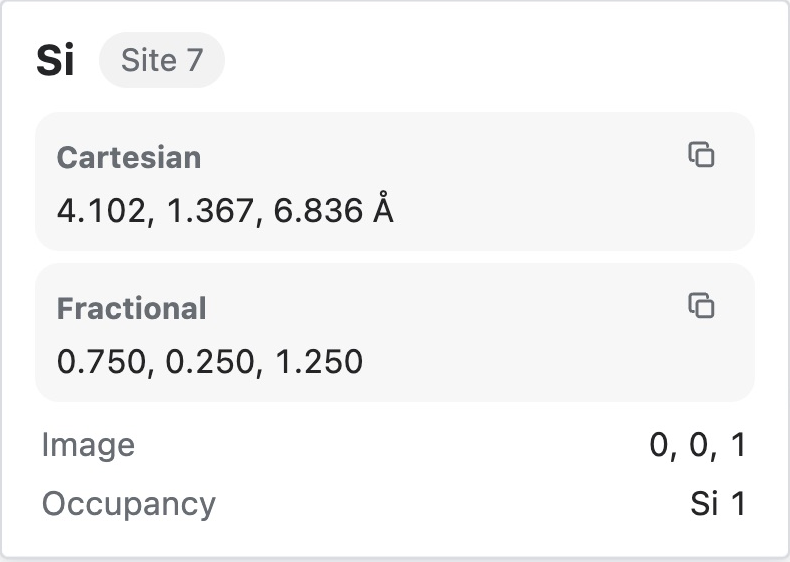
\includegraphics[width=79mm]{publication-assets/crop-4ce96785f91c44d963be.png}
\caption{Site 7週期映像的原子資訊卡區域性。分數座標和映像偏移應一起閱讀；該原子仍屬於模型的第7個位點。\ui{Occupancy}中的Si 1表示該位點由矽完全佔據。}
\label{fig:si-periodic-image-inspection}
\end{figure}

\subsection{顯示更多晶胞}

有時，一個晶胞不足以看清晶體中的連續連線。在三維檢視自己的工具欄開啟檢視器設定，找到 \ui{Repeat cell}，將 $a$、$b$、$c$ 三個方向分別設為\mbox{2、2、1}。檢視會顯示更多週期映像，從而更容易辨認空間排列。觀察完成後，可使用恢復按鈕回到 $1\times1\times1$。

這項設定只控制顯示重複範圍。它不會把專案中的 8 原子結構變成一個用於計算的更大模型。需要模擬局域缺陷或降低週期映像之間的相互影響時，應使用後面的\ui{構建超胞}命令。兩者雖然都可能讓螢幕上出現更多原子，改變的物件卻不同。

\subsection{調整表示方式}

球棍表示適合辨認連線關係，較大的原子半徑適合觀察原子佔據的空間。檢視器設定中可選擇元素配色、原子半徑方式和原子比例，控制化學鍵、晶胞邊框、配位多面體等物件的顯示。製作講義或報告時，先確定需要說明的問題，再選擇表示方式；同一張圖同時開啟所有輔助物件，往往會遮住需要觀察的區域性結構。

晶體中的化學鍵常由鄰近關係分析得到。改變成鍵策略後，顯示的鍵可能發生變化，而原子的實際位置沒有變化。對於具有明確拓撲的分子，應優先使用原始檔中的連線關係；對於晶體，應結合配位環境理解顯示結果。

\section{精確編輯原子}

\subsection{形成合適的選擇}

單擊可以選擇原子，按住 Shift 或 Ctrl 再單擊可以加入或移出當前選擇。雙擊可選擇相連結構。原子較多時，按 B 後拖動進行框選，按 L 後拖動進行套索選擇。按 Cmd/Ctrl+A 可全選，按 Esc 退出當前工具或清除選擇。

選擇並不一定等於螢幕上被圈住的所有球。例如，週期顯示可能包含同一個底層位點的不同映像。編輯前應檢視選擇數量和位點序號，尤其是在顯示重複範圍大於一個晶胞時。需要多次使用同一組位點，可將選擇儲存為選擇集，之後從\ui{選擇集}選單重新呼叫。

\begin{notebox}{為什麼 sites 與 atoms 不同}
檢視器摘要中的 \ui{sites} 表示模型的獨立位點數，\ui{atoms} 則包含用於顯示邊界和週期連線的原子映像。核對超胞倍數、元素計數或缺陷數量時，應以模型位點數為準。一個 8 位點矽晶胞可以顯示多於 8 個原子球；建立 $2\times2\times2$ 超胞後，應檢查 64 個位點，而不是要求螢幕上的原子球數量恰好等於 64。
\end{notebox}

\begin{figure}[htbp]
\centering
\begin{tikzpicture}[x=1mm,y=1mm,font=\sffamily\small]
  \node[text=brand] at (21,42) {模型：2 个独立位点};
  \node[text=brand] at (85,42) {视图：位点与映像};
  \fill[paleblue] (5,0) rectangle (37,32);
  \fill[paleblue] (69,0) rectangle (101,32);
  \draw[teal,line width=.75pt] (5,0) rectangle (37,32);
  \draw[teal,line width=.75pt] (69,0) rectangle (101,32);
  \fill[brand] (5,0) circle (2.3);
  \fill[teal] (21,16) circle (2.3);
  \node[text=white,font=\sffamily\scriptsize] at (5,0) {A};
  \node[text=white,font=\sffamily\scriptsize] at (21,16) {B};
  \fill[brand] (69,0) circle (2.3);
  \fill[teal] (85,16) circle (2.3);
  \node[text=white,font=\sffamily\scriptsize] at (69,0) {A};
  \node[text=white,font=\sffamily\scriptsize] at (85,16) {B};
  \foreach \x/\y in {101/0,69/32,101/32} {
    \draw[fill=white,draw=brand,line width=.8pt] (\x,\y) circle (2.3);
    \node[text=brand,font=\sffamily\scriptsize] at (\x,\y) {A};
  }
  \draw[->,>=stealth,teal,line width=.75pt] (43,16) -- (61,16);
  \node[text=brand,font=\sffamily\footnotesize] at (52,23) {周期显示};
  \node[text=ink,font=\sffamily\footnotesize,align=center] at (21,-8) {只保存 A、B 两个位点};
  \node[text=ink,font=\sffamily\footnotesize,align=center] at (85,-8) {空心圆是 A 的边界映像};
\end{tikzpicture}
\caption{独立位点与边界映像（二维示意）。同一位点 A 可以出现在多个周期边界上，绘制更多原子球并没有增加模型中的独立位点。}
\label{fig:periodic-sites}
\end{figure}


對需要嚴格指定順序的幾何操作，建議先清除選擇，再逐個點選。兩原子給出距離；三個原子定義以第二個原子為頂點的角；四個原子依次定義二面角。順序改變，幾何量的含義也可能改變。

\subsection{直接拖動與數值編輯}

選好原子後，按 G 再拖動可移動選擇，按 R 再拖動可旋轉選擇；變換過程中按 X、Y 或 Z 可以約束方向。直接拖動適合安排大致構型。若需要確定的位移、轉角或鍵長，應開啟對應引數命令，用數值完成最後一步。

\ui{平移原子}輸入的是位移向量，而\ui{移動原子}輸入的是新的座標。將一個原子從 $(1,0,0)$ 移到 $(2,0,0)$，可以給它平移 $(1,0,0)$，也可以把新座標設為 $(2,0,0)$。在晶體中，兩類命令還允許使用相應的分數或笛卡爾表示，輸入前應檢查座標選項。

\ui{旋轉原子}需要轉軸、角度和錨點。角度以度為單位；錨點是轉軸經過的位置。若希望一個片段繞自己的連線位點轉動，應把錨點放在連線位點附近，而不是沿用與片段相距很遠的原點。這樣，預覽中的運動更符合預期。

\section{提交結構修改}

大多數會改變結構的引數對話方塊都提供\ui{預覽}、\ui{應用}和\ui{取消}。預覽用於檢查引數的幾何效果；應用將修改寫入當前文件的編輯狀態；儲存再將該狀態寫回專案。修改引數後可重新預覽；取消則退出命令並恢復原檢視。

\begin{steps}
  \item 開啟需要的建模命令，核對當前選擇與引數單位。
  \item 輸入引數後單擊\ui{預覽}。轉動或縮放檢視，檢查模型中發生變化的部位。
  \item 若結果合適，單擊\ui{應用}；若不合適，修改引數重新預覽，或單擊\ui{取消}恢復原檢視。
  \item 應用後檢查原子數量、晶胞或幾何值。可用 Cmd/Ctrl+Z 撤銷，用 Shift+Cmd/Ctrl+Z 重做。
  \item 完成一段有意義的工作後儲存專案，併為模型保留清楚的名稱。
\end{steps}

\ui{歷史}區域中的\ui{重置}恢復開啟當前文件或最近儲存時的結構。它與重新居中相機的按鈕不同。儲存後，最近儲存的模型會成為新的編輯基準，當前撤銷歷史隨之清空；如果希望長期比較兩套模型，應保留兩個有明確名稱的專案結構，而不要只依賴撤銷記錄。

純分析命令不一定產生新的結構預覽，結果的顯示方式也因命令而異。\ui{分子診斷}按規則檢查當前分子的價態、近距離接觸和鍵長，不改變結構；圖形介面完成後顯示\ui{Molecule diagnostics completed.}。檢查結果時，結合分子組成、連線和幾何讀數進行判斷。具體檢查方法見本章\ref{sec:molecule-manual-check}節；MATLAB\regmark{}工具箱使用者還可透過配套指令碼讀取診斷資料。

\section{示例：矽超胞與一個空位}

\subsection{把晶胞擴大為超胞}
\index{Chaobao@超胞}

超胞把基本晶胞沿選定方向複製，並把複製得到的全部原子作為新模型的一部分。對於對角重複 $(n_x,n_y,n_z)$，原子數和體積均擴大 $n_xn_yn_z$ 倍。本例從 8 位點矽晶胞建立 $2\times2\times2$ 超胞，因而模型應包含 64 個獨立位點。這個數量由輸入檔案和重複倍數確定，可用來檢查操作。

\begin{steps}
  \item 回到由 \file{Si.poscar} 匯入的 \file{Si} 文件，將顯示重複恢復為 $1\times1\times1$，避免把顯示映像與模型原子混淆。
  \item 在頂部\ui{晶體建模}的\ui{晶體與晶胞}區域開啟\ui{超胞與晶格}，選擇\ui{構建超胞}。
  \item 在\ui{超胞倍率或變換矩陣}中核對預設的 \literalinput{2 2 2}，單擊\ui{預覽}。從晶胞邊框觀察三個方向的擴大；視窗下方會提示預覽已顯示。
  \item 確認預覽合適後，單擊\ui{應用}。
  \item 檢查模型有64個矽位點，三個晶格向量長度分別為原來的兩倍。圖中的摘要顯示64 sites、166 atoms；核對擴胞倍數時看前者。如需長期保留無缺陷超胞，可以在繼續建立空位前另存一個專案副本。
\end{steps}

一般超胞由一個整數矩陣 $S$ 定義。矩陣的每一行說明一條新晶格向量由原來的三條向量怎樣組合。例如，第一行為 $(2,1,0)$，就表示 $\mathbf a'=2\mathbf a+\mathbf b$。在本書的行向量約定下，晶格、體積和位點數滿足
\begin{equation}
 A'=SA,\qquad V'=|\det S|V,\qquad N'=|\det S|N.
 \label{eq:supercell-count-volume}
\end{equation}
$S$ 中的數必須是整數，且行列式不能為零。$|\det S|$ 是新舊晶胞的體積比，也是獨立位點數的倍數；$N$ 始終數模型位點，不數邊界上額外繪出的原子映像。對於三個重複數，$S=\operatorname{diag}(n_a,n_b,n_c)$，式\eqref{eq:supercell-count-volume}就回到三個重複數相乘的規則。前面的矽超胞例子取 $S=2I$，所以 $|\det S|=8$，8個位點變為64個。

下面用一個非對角矩陣作代數檢查：
\[
 S=\begin{bmatrix}2&1&0\\0&1&0\\0&0&1\end{bmatrix},\qquad
 \begin{cases}
 \mathbf a'=2\mathbf a+\mathbf b,\\
 \mathbf b'=\mathbf b,\quad \mathbf c'=\mathbf c.
 \end{cases}
\]
其行列式為2。若原模型含8個位點，新模型應含16個位點，體積是原來的兩倍；新外框可以傾斜，週期材料本身的區域性排列仍來自原結構的複製。這與透過應變拉伸原子間距有區別：超胞選擇更大的重複單元，不把每條原子間連線都拉長兩倍。

在\ui{超胞倍率或變換矩陣}中，可以填寫三個重複整數，也可以填寫完整的 $3\times3$ 矩陣。使用一般矩陣前先寫出三條新基矢，再檢查行列式、預覽外框和應用後的位點數，便不容易把“重新定向”和“增加了多少原子”混為一談。輸入\literalinput{1 1 1}時，矩陣為 $I$，模型不擴大；本工具仍會把等價座標歸入單位晶胞，適合將落在胞外的代表位置整理到同一胞中檢視。


\begin{figure}[!htb]
\centering
% 原图3024×1758；完整窗口(670,585,2355,1455)，1685×870；122mm约351ppi。
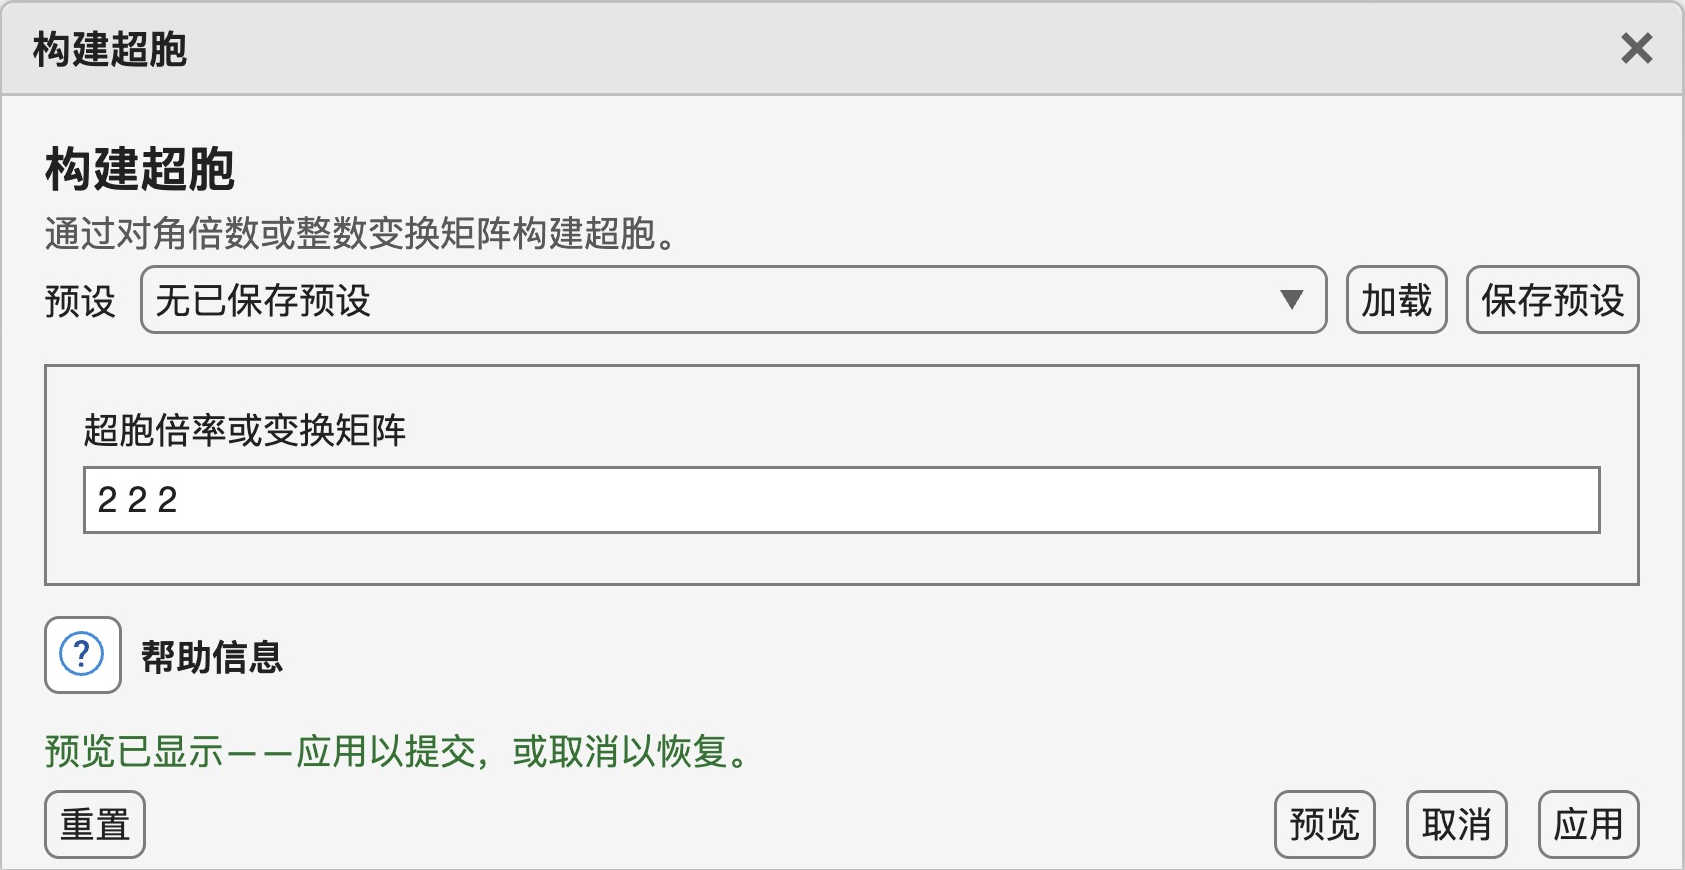
\includegraphics[width=\linewidth]{publication-assets/crop-0ff9d4164c5629316893.png}
\caption{構建超胞的引數與預覽狀態。\literalinput{2 2 2}表示三個方向分別重複兩次。}
\label{fig:si-supercell-preview}
\end{figure}

\begin{figure}[!htb]
\centering
\begin{minipage}[b]{78mm}
% 原图3024×1758；完整模型(875,365,2155,1615)，1280×1250；78mm约417ppi。
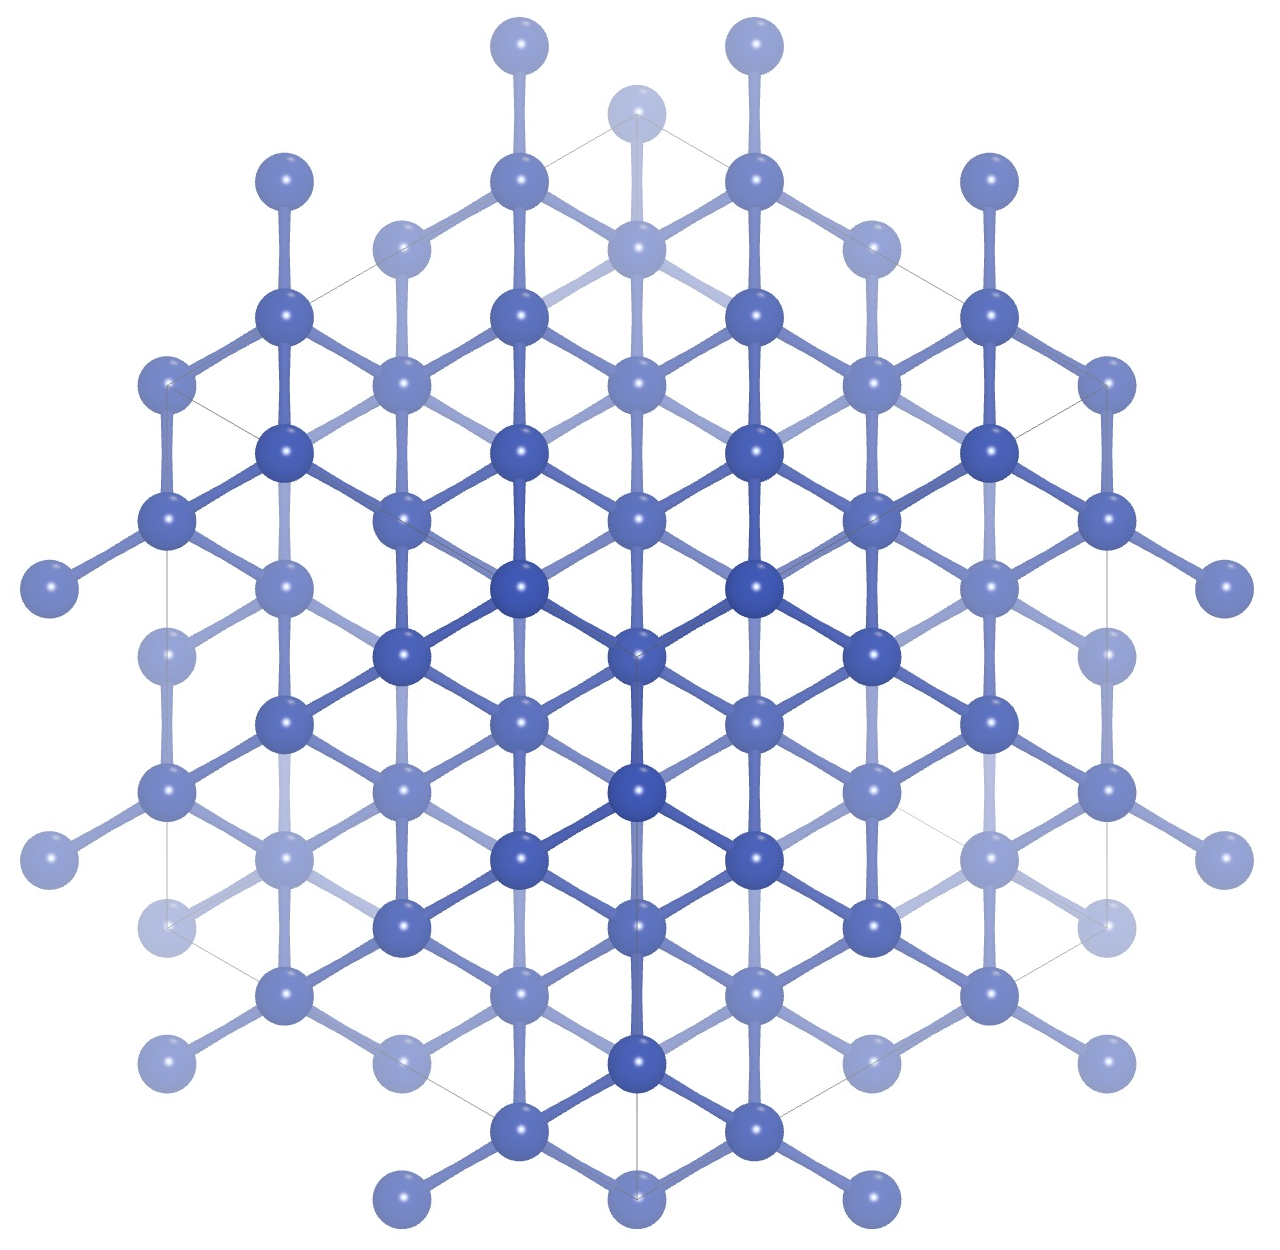
\includegraphics[width=\linewidth]{publication-assets/crop-0469f894473f746988e3.png}
\end{minipage}\hfill
\begin{minipage}[b]{42mm}
% 同图独立摘要(45,330,465,560)，420×230；42mm约254ppi。
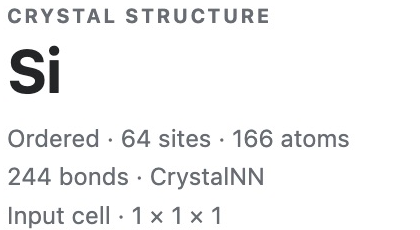
\includegraphics[width=\linewidth]{publication-assets/crop-c0154093dad09f77a9a2.png}
\end{minipage}
\caption{應用後的矽超胞，分別呈現完整模型與摘要區域性。64 sites是模型獨立位點數，166 atoms包含邊界映像；\ui{Input cell $1\times1\times1$}是對新超胞的顯示範圍。}
\label{fig:si-supercell-result}
\end{figure}

\subsection{建立並檢查空位}
\index{Kongwei@空位}

空位表示從晶格中的一個位點移去原子。建立空位前先擴大晶胞，可以減小相鄰週期映像之間的距離過近所帶來的影響；具體需要多大超胞，應結合後續計算的收斂檢查決定。缺陷形成能可在模型建立後透過相應計算求得。

\begin{steps}
  \item 確認當前活動文件仍是剛建立的64位點 \file{Si} 超胞。本例移去原子序號1。
  \item 在\ui{晶體建模}的\ui{晶體材料}區域開啟\ui{缺陷與合金}，依次選擇\ui{建立點缺陷 → 空位}。在引數視窗核對\ui{缺陷型別}為\ui{空位}，\ui{原子序號（從 1 開始）}輸入\file{1}。
  \item 核對型別和序號後單擊\ui{應用}。轉動檢視，觀察移去原子後鄰近位置的連線。
  \item 檢查位點數由64變為63，晶胞仍是所建立的超胞。本例摘要為63 sites、162 atoms；顯示映像減少的數量不必等於移去的獨立位點數。
  \item 使用\ui{另存為}儲存為\file{Si-vacancy-tutorial.ks}，保留原來的\file{Si-introduction.ks}。儲存後檢查標題中的未儲存星號已消失。
\end{steps}

\begin{figure}[!htb]
\centering
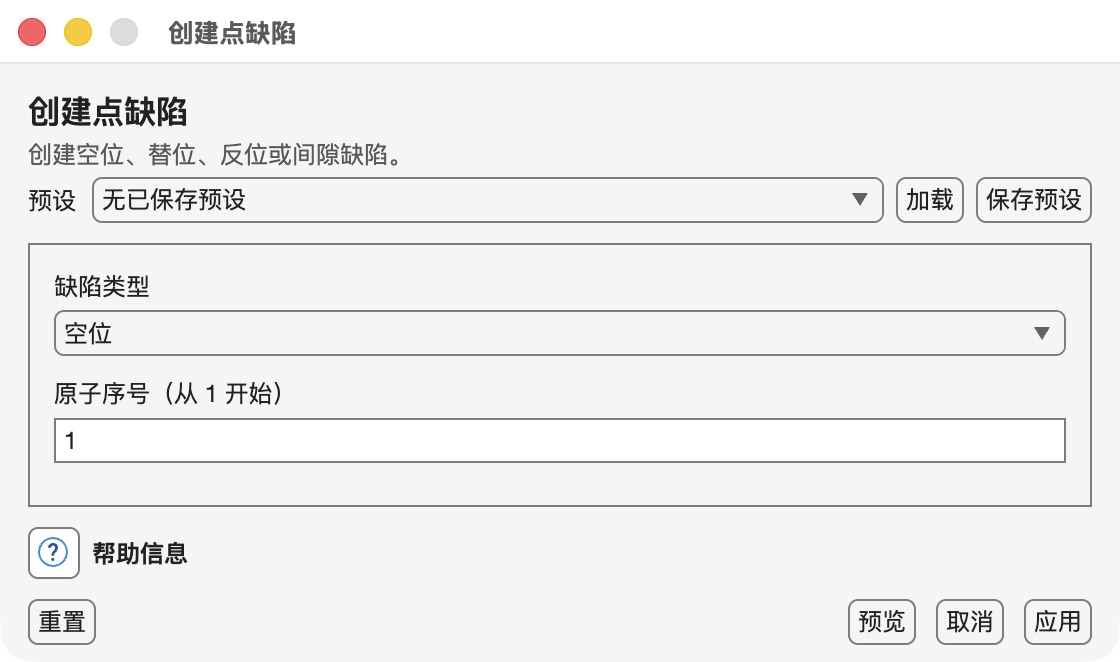
\includegraphics[width=113.7mm]{publication-assets/crop-601f9ce2a238baeb7b2e.png}
\caption{建立矽空位的引數。缺陷型別為\ui{空位}，原子序號為1；應用後按正文檢查獨立位點由64減為63。}
\label{fig:si-vacancy-settings-result}
\end{figure}

隨書的\file{Si-vacancy-tutorial.ks}包含原來的\file{silicon}對照結構和完成空位編輯的\file{Si}結構。需要無缺陷超胞作對照時，可從\file{Si.poscar}按上述步驟重新建立64位點模型，並在建立空位前另存。

晶體原子編輯中的對稱性處理會影響等價位置。如果目的是局域缺陷，應明確自己需要的是單個位點變化，還是整組等價位點的變化。\ui{建立點缺陷}提供了直接表達空位、替位、間隙和反位的入口，應用後按獨立位點數與元素計數檢查結果。

\section{示例：從芳香環建立苯和吡啶}
\index{Fangxiang fenzi@芳香分子}

\subsection{建立苯分子的骨架}

分子草繪可以在三維檢視中逐個放置原子，也可以用環和片段快速建立骨架。按 S 進入草繪後，單擊空白處放置獨立原子，從已有原子拖動可新增相連原子，拖向另一已有原子可建立連線。草繪欄用於選擇元素、鍵級和環。

本例先透過引數命令建立規則六元環，便於理解芳香性和加氫的作用。

\begin{steps}
  \item 選擇\ui{主頁 → 結構 → 新建結構 → 空白分子結構}，啟用新文件，在\ui{分子建模}中開啟\ui{繪製環}。
  \item 環尺寸設為 6，元素為 C，邊長為 $1.4\,\text{\AA}$，啟用芳香環。中心的三個數值框分別填 0、0、0；法向的三個數值框分別填 0、0、1。
  \item 保持不連線到其他原子，預覽並應用。此時得到碳骨架，尚需補足氫。
  \item 按 Cmd/Ctrl+A 選中六個環原子，執行\ui{新增氫}。檢查應形成苯的組成 $\mathrm{C_6H_6}$。
  \item 執行\ui{分子診斷}，關閉完成提示。旋轉檢視，檢查六元環、每個碳相連的氫和區域性距離，再儲存模型，命名為\file{Benzene}。
\end{steps}

芳香環的連線資訊與普通單鍵環不同。僅把六個碳擺成六邊形，或僅讓顯示的鍵看起來相同，都不能替代芳香鍵和原子化學性質的設定。檢查模型時，應同時觀察分子組成、鍵級與芳香標記。

補氫後還應轉到側面檢查整個分子。環骨架共面，並不表示自動放置的氫已經落在環平面內。隨書的\file{benzene.json}保留本例補氫後的初始狀態，\mbox{\file{benzene-optimized.json}}保留通用分子模型最佳化後的狀態，便於對照；後者仍是建模參考結構。需要單獨交換這些芳香分子時，可使用原生 JSON 儲存化學屬性與芳香鍵，並在重新匯入後核對連線。

\subsection{把一個碳改為氮}

先儲存當前苯模型，再選擇\ui{主頁 → 結構 → 從檔案匯入結構…}，再次匯入隨書\file{benzene.json}，開啟新匯入的結構，用它練習吡啶。這樣可以保留原來的苯作為對照。為使加氫過程清楚，先移除氫，再替換環上的一個碳。

\begin{steps}
  \item 在新匯入的結構中全選並執行\ui{刪除氫}，隨後選擇一個環碳，開啟\ui{原子化學屬性}。
  \item 將元素改為 N，形式電荷為 0，雜化設為 \file{sp2}，保持芳香原子選項。
\end{steps}

% Online实机吡啶示例；由主控插入第7章适当位置。
% 仅以LaTeX矩形裁切原JPEG，不修改、拼接或重绘像素。
\begin{figure}[H]
\centering
% 原图3024×1758；参数范围(710,735,2315,1585)，1605×850，122mm约334ppi。
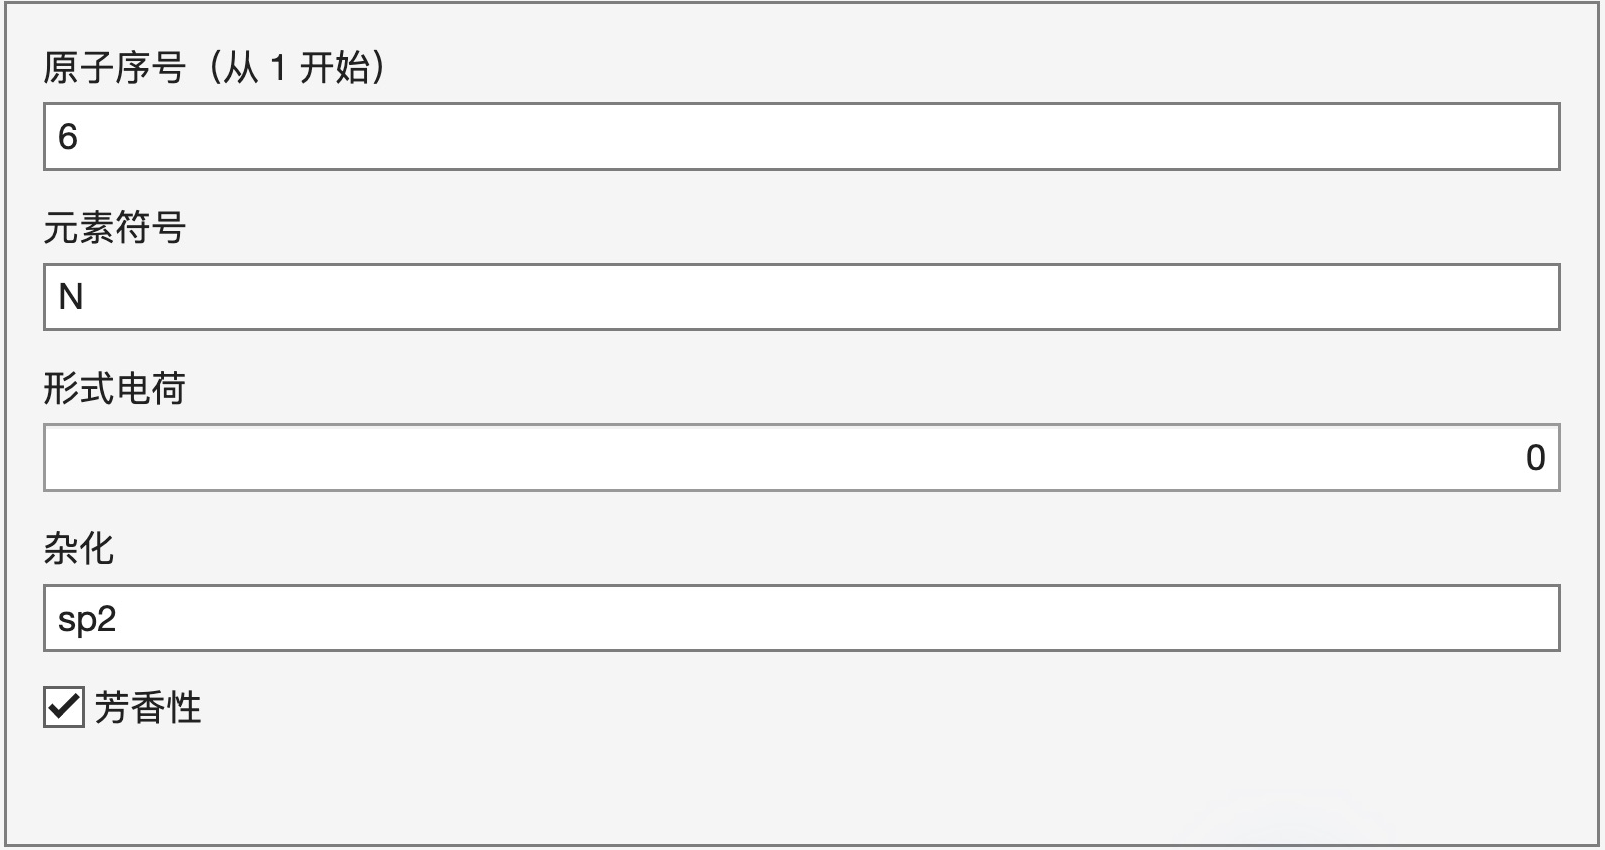
\includegraphics[width=\linewidth]{publication-assets/crop-f99354db0f163eccfd81.png}
\par\vspace{2mm}
% 同一原图的独立预览提示范围(700,1615,1520,1670)，820×55；排除右侧指针。
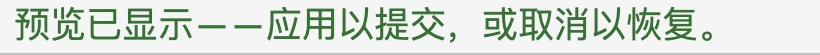
\includegraphics[width=80mm]{publication-assets/crop-8ce96edd826deccee006.png}
\caption{将环上第6个原子替换为氮的参数：元素为N，形式电荷为0，杂化为\ui{sp2}，勾选\ui{芳香性}。下方显示预览提示，单击\ui{应用}提交修改。}
\label{fig:pyridine-chemistry}
\end{figure}


\begin{steps}[resume]
  \item 應用後全選環原子並\ui{新增氫}，檢查組成應為 $\mathrm{C_5H_5N}$，並檢查氮附近的連線。
  \item 執行\ui{分子診斷}，關閉完成提示後，回到檢視比較苯與吡啶的組成、環連線和氮附近的氫數。可匯入隨書\file{pyridine.json}，對照完整的中性吡啶模型。
\end{steps}

形式電荷、雜化提示與元素共同影響連線關係的解釋。若替換元素後繼續沿用原先全部氫原子，可能得到與預期不同的價態。對於這類修改，先處理骨架再補氫，通常更容易檢查。

中性吡啶有 42 個電子，本例採用單重態。從含奇數電子的骨架繼續加氫時，可能保留骨架的自旋多重度，導致再次讀取檔案時提示電荷與自旋不匹配。隨書\file{pyridine.json}的電荷為 0、多重度為 1；需要繼續計算時，可以從這份檔案開始。

圖\ref{fig:pyridine-chemistry}顯示將第6號環原子改為氮的引數；圖\ref{fig:pyridine-built-model}可用於核對補氫後的六元環和五個氫原子。

% 吡啶应用和补氢后的结果，接在读者检查步骤之后。
\begin{figure}[H]
\centering
% 原图3024×1758；几何范围(900,370,2120,1680)，1220×1310；70mm约443ppi。
% 不包含摘要；当前会话保留骨架多重度的现象由第7章正文另行说明。
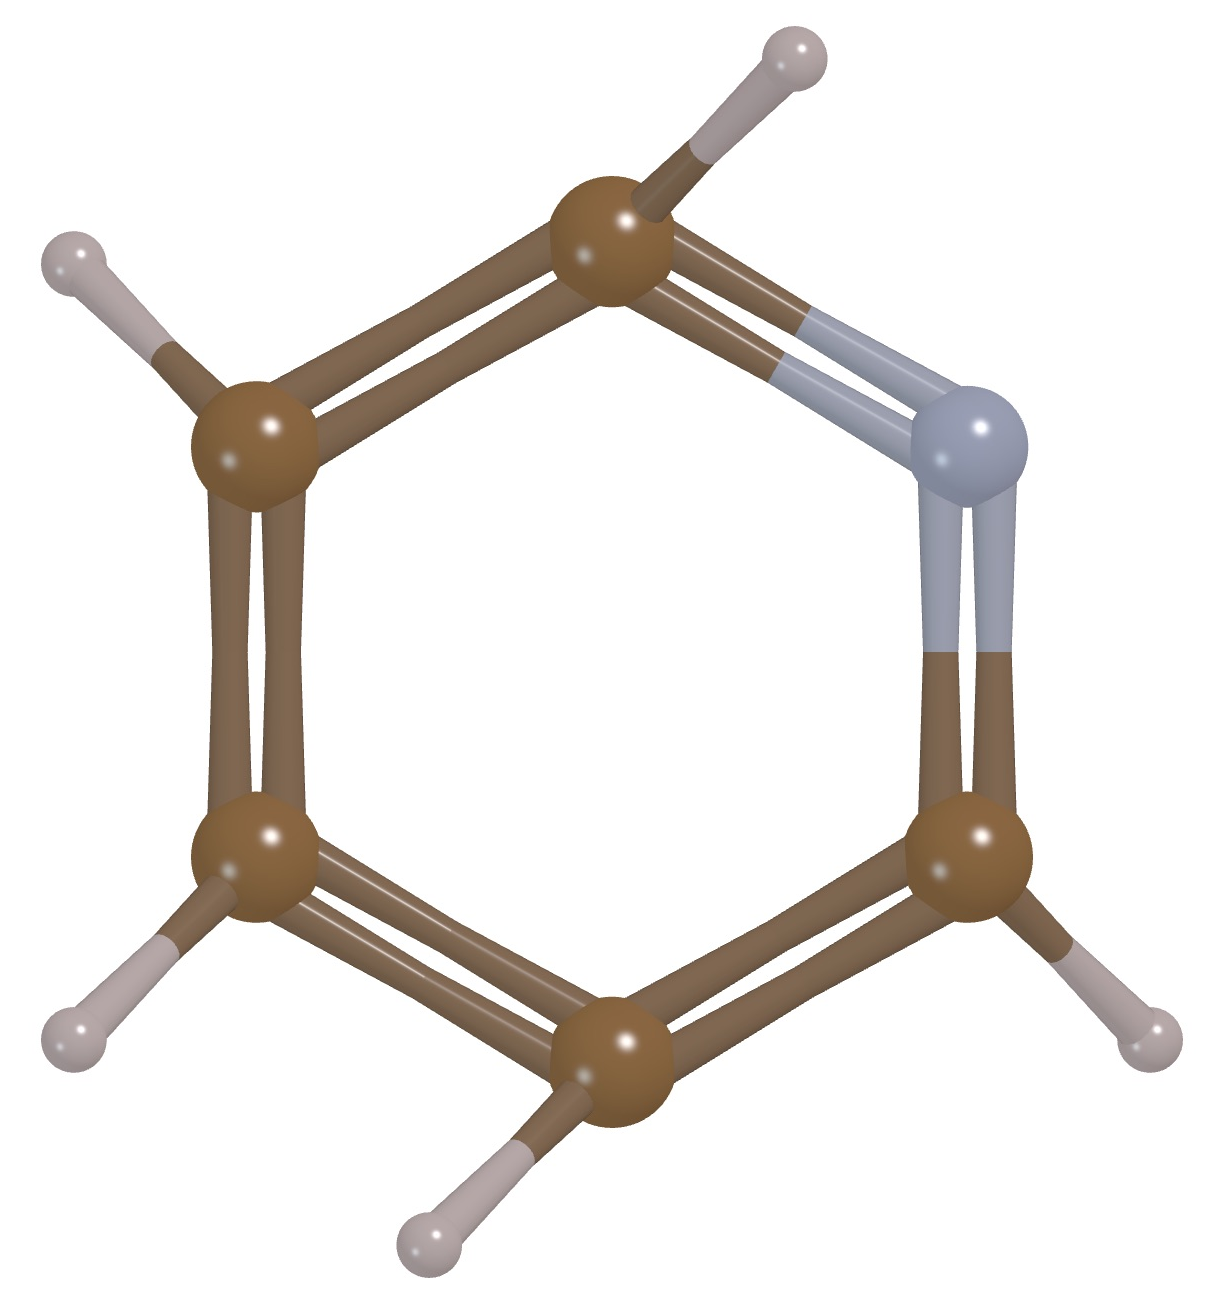
\includegraphics[width=70mm]{publication-assets/crop-60c8057a2bb7c31f0fd8.png}
\caption{完成元素替换并对六个环原子补氢后的吡啶初始结构：五个碳、一个氮和五个氢，共11个原子、11条连接。继续计算时，可使用随书\file{pyridine.json}中的中性单重态结构。}
\label{fig:pyridine-built-model}
\end{figure}


\section{示例：調整乙醇構象}
\index{Fenzi jihe@分子幾何}

\subsection{建立連線清楚的初始分子}

乙醇的重原子骨架是 C--C--O。先選擇\ui{主頁 → 結構 → 新建結構 → 空白分子結構}，開啟新文件，再依次草繪三個原子並新增氫；也可以透過新增原子和建鍵命令完成。為了使輸入便於核對，本例使用以下初始座標，長度單位為 \AA。

\begin{table}[htbp]
\centering
\caption{乙醇骨架的練習輸入。共線座標只用於開始幾何編輯。}
\begin{tabularx}{\linewidth}{lX}
\toprule
原子與序號 & 輸入與連線 \\
\midrule
1：C & 座標 $(0,0,0)$；作為第一個獨立原子。\\
2：C & 座標 $(1.52,0,0)$；與原子 1 以單鍵連線。\\
3：O & 座標 $(2.95,0,0)$；與原子 2 以單鍵連線。\\
\bottomrule
\end{tabularx}
\end{table}

當草繪命令啟用了\ui{使用力場理想鍵長}時，工具會按連線方向採用理想鍵長。需要嚴格使用表中的練習座標時，關閉這一選項。骨架建立後補氫，檢查組成應為 $\mathrm{C_2H_6O}$。這一初始構型還沒有經過幾何整理，不宜將其中的共線骨架當成乙醇的穩定構型。

\subsection{設定幾何量}
\index{Juli@距離測量}
\index{Jianjiao@鍵角}
\index{Ermianjiao@二面角}

需要讀取距離時，在三維檢視工具欄的\ui{Measurements}中選擇\ui{Atom-to-atom distance}，再依次單擊原子1、2。要修改距離，開啟頂部\ui{設定距離}，在原子序號中填\literalinput{1 2}，把目標設為$1.52\,\text{\AA}$。接著開啟\ui{設定鍵角}，原子序號填\literalinput{1 2 3}，目標填$109.5^\circ$。本例的距離、鍵角和二面角操作均選擇\ui{子樹}移動範圍，使相連的原子一起調整。

\ui{原子}範圍只移動區域性原子；\ui{子樹}沿連線關係移動一側；\ui{片段}用於對一個連線片段整體調整。改變鍵角時，如果只移動一個重原子而沒有帶動其相連氫，附近幾何可能變差。預覽時應把整個分子納入觀察，而不要只看目標角的數值。

\begin{steps}
  \item 對 C--C--O 骨架設定需要的距離和角度，每次應用後重新測量一次。
  \item 調整檢視，按需要依次選擇四個相連原子，例如 C--C--O--H。確認最後一個是與 O 相連的氫。
  \item 在\ui{設定二面角}中輸入一個便於比較的角度，例如 $60^\circ$，使用預覽觀察末端片段的轉動。
  \item 換用另一二面角後再次觀察，並用撤銷返回前一構型。透過這一對比理解構象變化，而不是把某個輸入角度直接解釋為能量最低構象。
\end{steps}

\subsection{在檢視器中核對鍵角}

幾何編輯後的數值，可在三維檢視自己的測量卡片中讀取。頂部\ui{幾何編輯 → 測量幾何}是另一個命令；圖形介面完成後顯示\ui{Geometry measurement completed.}，不在提示框中列出數值。需要檢查角度時，按下面的檢視器步驟操作。

圖\ref{fig:ethanol-angle-parameters}與圖\ref{fig:ethanol-angle-measured}展示鍵角的設定與測量。為便於選擇原子，本節從隨書\mbox{\file{ethanol-optimized.json}}匯入副本，再修改指定角度；它與前面從共線骨架逐步建立分子的過程採用不同的起點。

\begin{steps}
  \item 匯入\mbox{\file{ethanol-optimized.json}}，開啟副本的分子文件，保留原檔案作為參考。
  \item 在\ui{設定鍵角}中填寫原子\literalinput{1 2 3}、目標$109.5^\circ$與\file{subtree}移動範圍，先預覽，再應用。這一操作直接設定幾何量，後續可繼續進行分子最佳化。
\end{steps}

% Online实际乙醇设置/测量；只以LaTeX裁切原生JPEG，不修改像素。
\begin{figure}[H]
\centering
% 原图3024×1758；(710,820,2310,1400)，1600×580，122mm约333ppi。
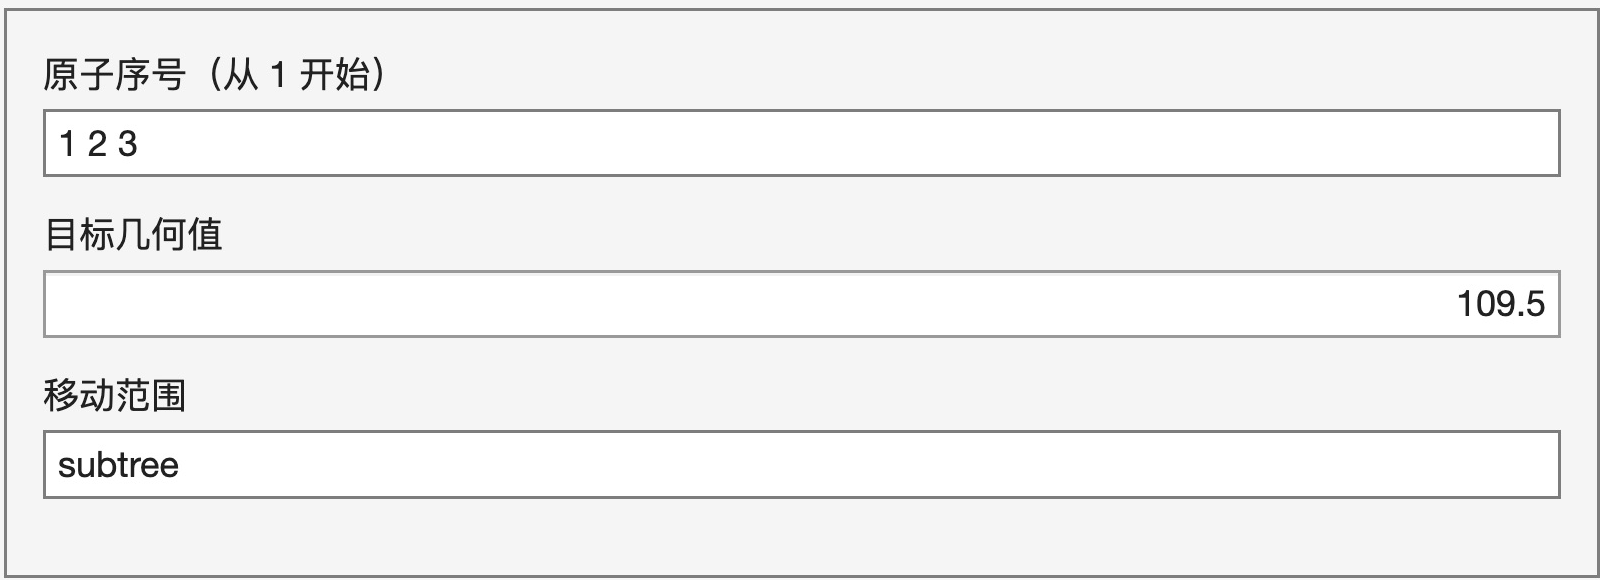
\includegraphics[width=\linewidth]{publication-assets/crop-0483f84ce4963946e315.png}
\par\vspace{2mm}
% 独立状态局部(710,1425,1520,1482)，810×57；去掉上方指针及下方按钮边缘。

\includegraphics[width=80mm]{publication-assets/crop-17309e4ada4dd6ce532b.png}
\caption{设置乙醇键角的参数。按顺序输入原子\literalinput{1 2 3}，目标为$109.5^\circ$，移动范围为\file{subtree}；下方显示预览提示，单击\ui{应用}提交修改。}
\label{fig:ethanol-angle-parameters}
\end{figure}


\begin{steps}[resume]
  \item 關閉引數視窗，在三維檢視右側工具欄找到尺形的\ui{Measurements}按鈕，選擇\ui{Bond angle}。進入測量後，按新的順序重新點選原子。
  \item 依次單擊1號C、2號C、3號O，第二個原子是角的頂點。圖中1號C在上方，2號C在中間，O為紅色。完成第三次點選後，左側測量卡片顯示角度和原子路徑，模型中出現兩條角邊與圓弧。
  \item 核對卡片為$109.500^\circ$，路徑為\ui{\#1 C}、\ui{\#2 C}、\ui{\#3 O}。記下測量值與原子順序，關閉結果卡片，再儲存修改後的副本。
\end{steps}

這個讀數表明幾何編輯已得到指定角度；乙醇的平衡鍵角需由最佳化計算確定。需要比較最佳化前後時，應對兩份分別儲存的模型採用同一原子順序測量，並記錄各自實際讀數。

% 乙醇实际测量结果，接在查看器点选与读数步骤之后。
\begin{figure}[H]
\centering
\begin{minipage}[t]{62mm}
\vspace{0pt}
% 测量卡片(55,328,845,1717)，790×1389；62mm约324ppi。
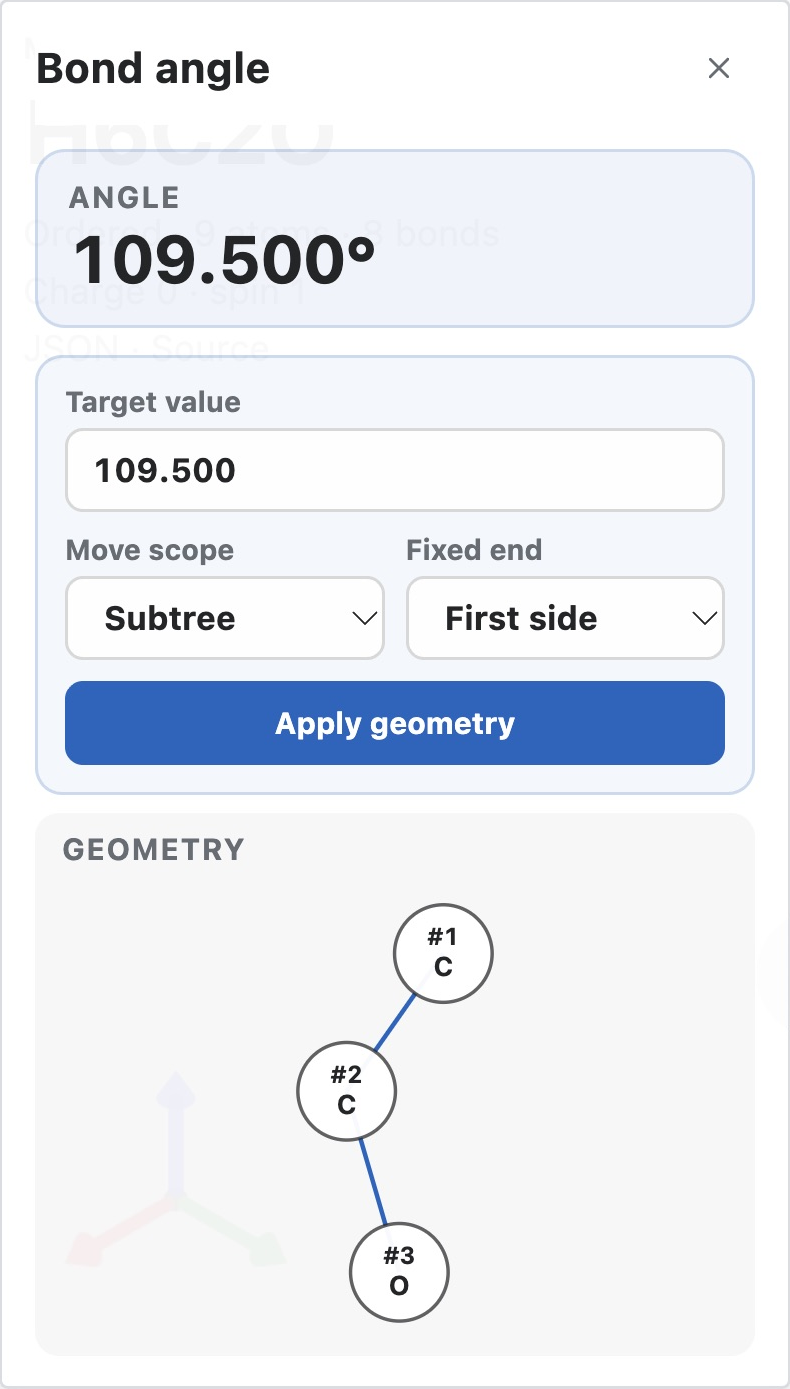
\includegraphics[width=\linewidth]{publication-assets/crop-cdb0f92bdcdbb307f144.png}
\end{minipage}\hfill
\begin{minipage}[t]{58mm}
\vspace{0pt}
% 三重原子和实际角线(850,400,2000,1650)，1150×1250；58mm约504ppi。
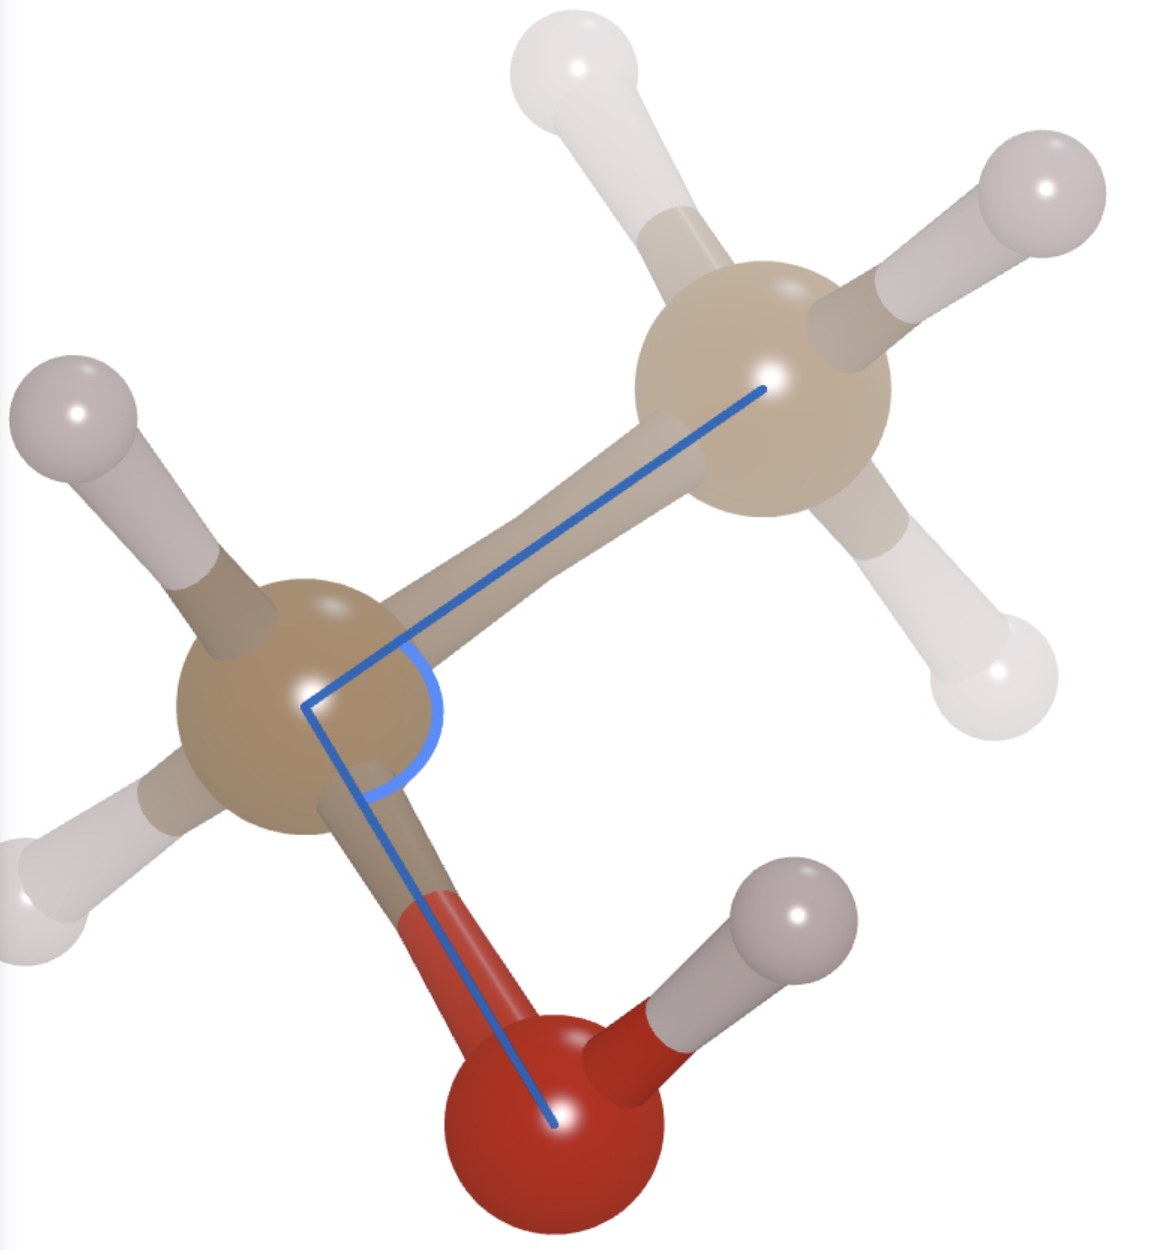
\includegraphics[width=\linewidth]{publication-assets/crop-4185f48c89b2b877f7b1.png}
\end{minipage}
\caption{使用查看器\ui{Bond angle}测量设置后的键角。左侧读数为$109.500^\circ$，路径为\#1 C、\#2 C、\#3 O；右侧显示三个重原子和角线。练习从\file{ethanol-optimized.json}的副本开始，将该角设为$109.5^\circ$；此数值为练习的目标角度。}
\label{fig:ethanol-angle-measured}
\end{figure}


\subsection{整理與最佳化幾何}

\ui{整理幾何}使用規則改善明顯的區域性幾何問題；\ui{最佳化幾何}在通用分子模型下進一步調整結構。它們適合準備初始分子，尤其是手工草繪或改動連線之後。最佳化引數包括最大迭代次數、力收斂容差，以及可選的固定原子序號。

可以先使用預設的最多200次迭代和0.001力容差，預覽並應用後，比較結構變化，再測量關注的鍵長、鍵角和近距離接觸。配套指令碼提供最佳化方法與收斂過程的詳細記錄。後續若要研究精確的平衡幾何、構象能量或反應過程，應在計算章節所述的合適方法下繼續處理。

隨書\file{ethanol-edited.json}保留本例的幾何編輯結果，重新匯入後測得 C--C 距離 $1.52\,\text{\AA}$、C--C--O 鍵角 $109.5^\circ$，以原子 9 為末端氫的 C--C--O--H 二面角為 $60^\circ$。\mbox{\file{ethanol-optimized.json}}則經過整理和通用分子模型最佳化：該參考結構經 47 次迭代達到 $0.001\,\mathrm{kJ/(mol\,\text{\AA})}$ 的力閾值。最佳化允許這些幾何量繼續改變，因此不能把編輯時指定的數值當作最佳化後仍然固定的約束。

\subsection{核對分子的組成和幾何}\label{sec:molecule-manual-check}

在圖形介面中，可以按下面的順序檢查編輯結果，並把前後讀數記在一起。

\begin{steps}
  \item 檢視結構摘要中的分子式和原子數，與計劃建立的分子比較。例如，苯應為$\mathrm{C_6H_6}$，吡啶應為$\mathrm{C_5H_5N}$，乙醇應為$\mathrm{C_2H_6O}$。
  \item 旋轉模型，逐個檢視發生修改的重原子及其相連的氫。結合已設定的元素、形式電荷、鍵級與芳香性判斷連線是否合理。需要更正時，選中對應原子，使用\ui{原子化學屬性}或\ui{設定鍵級}重新明確設定，再按連線補氫。
  \item 對可疑的短接觸，在檢視器的\ui{Measurements}中選擇\ui{Atom-to-atom distance}並依次點選兩個原子；檢查鍵角時選擇\ui{Bond angle}並依次點選三個原子。比較修改前後的實際讀數，避免只憑球體大小判斷原子是否過近。
  \item 儲存模型及檢查記錄。需要檢視顯式鍵和原子屬性的完整記錄時，匯出原生JSON；需要逐項診斷資料時，在MATLAB\regmark{}工具箱環境中執行配套檢查指令碼。
\end{steps}

\ui{分子診斷}檢查整個分子，診斷範圍不受區域性選擇限制。比較修改前後的結構時，使用組成、連線與幾何測量記錄。

\section{複用建模內容}

完成一個分子後，不必每次從單原子重新開始。先選擇連線位點，在頂部\ui{分子建模}頁面的同名下拉選單中開啟\ui{片段草繪器}，再選擇片段與連線模式，使用視窗中的\ui{連線片段}把片段接到模型。連線前核對片段名稱與連線頭。使用者片段可將經常使用的區域性結構儲存在庫中，重複單元則供高分子構建使用，二者用途不同。

引數對話方塊中的預設用於儲存常用引數。例如，某個超胞變換或表面厚度組合可以儲存為有意義的預設，下次載入後再按當前模型調整。載入預設後，按當前材料調整數值。選擇集則儲存一組位點，便於再次選取。

較長的一系列操作可使用\ui{錄製}與\ui{儲存 Recipe}保留建模過程。整理工作記錄或進行團隊協作時，記錄原始結構、操作引數和最終檔案，比只儲存一張三維截圖更容易複查。影象負責說明結構，模型檔案負責保留原子和晶胞；兩者共同組成一份完整的建模結果。
